\chapter{Introduction}
\label{intro}

\begin{itemize}
\item Gov Linkedata, Spatial data and visualizations
\item Evolution of LOD cloud: 2014, 2011, 2007
\item Percentage of geodata on the LOD Cloud
\end{itemize}

\section{Context}
\label{sec:context}

The Web of Linked Data is continuously evolving, started in 2007 with a dozen of datasets (cf. Figure\ref{fig:lodcloud2007}) to a large data space with thousands of datasets in different topics. From 2011 (See Figure \ref{fig:lodcloud2011})\cite{jentzsch2011} to 2014, there has been a significant growth of nearly $271\%$ of datasets depicted in the LOD cloud \cite{max2014}. The new version altogether contains 570 linked datasets which are connected by 2909 linksets, as depicted in Figure \ref{fig:lodcloud2014}\footnote{A more web friendly version can be accessed at \url{http://data.dws.informatik.uni-mannheim.de/lodcloud/2014/}}. In order to enable
Linked Data applications to discover datasets as well as to ease the integration of data from multiple sources, Linked Data publishers should comply with a set of best practices for publishing datasets on the web \cite{Heath2011}:

\begin{itemize}
\item \todo{add here part of BP doc of GLD group}

\item Vocabulary Usage: The best practices advise publishers to use terms from
widely-used vocabularies in order to ease the interpretation of their data. If data providers use their own vocabularies, the terms of such proprietary vocabularies.

\item Linking: By setting RDF links, data providers connect their datasets into a single global data graph which can be navigated by applications and enables the discovery of additional data by following RDF links.

\item Dereferencable URIs:  

\item Metadata Provision: 
\end{itemize}



\begin{figure}[ht!]
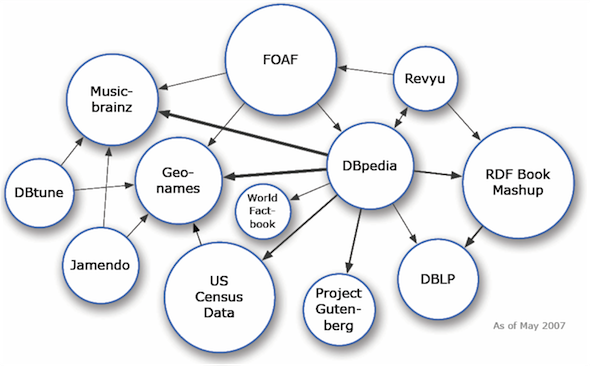
\includegraphics[scale=0.9]{img/lod-cloud2007.png}
\caption{LOD cloud as of May, 2007}
\label{fig:lodcloud2007}
\end{figure}

\begin{figure}[ht!]
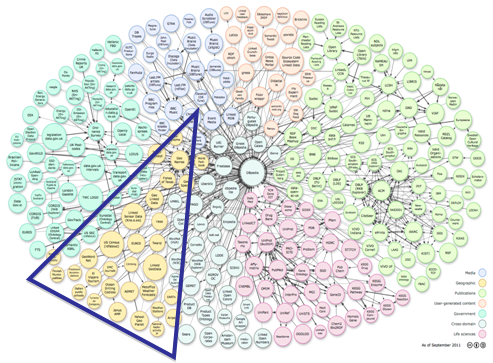
\includegraphics[scale=0.9]{img/lod-diagram-2011.png}
\caption{LOD cloud as of August, 2011}
\label{fig:lodcloud2011}
\end{figure}

\begin{figure}[ht!]
\centering{
\includegraphics[scale=0.1]{img/LODcloud2014.pdf}
\caption{LOD cloud as of April, 2014}
\label{fig:lodcloud2014}
}
\end{figure}



\section{Research Questions}
\label{sec:questions}

The Web is currently in a transition phase. After having been accessible on personal computers, it is now 
quickly moving to more and more ubiquity and entering in every part and moment of our lives. New 
devices and new ways to use them are being created. The ubiquity of the Web also creates an unseen 
abundance of information. Data is flowing onto the Web, created by users, generated by sensors, and 
stored in ever growing data farms. Geographic data is widely present on the web as they are used for location 
of Point of Interest. At the same time, many organizations are moving from legacy data stored in their databases
to structured data on the web. Structured data is already present in the many databases, metadata attached to medias, and in the millions of spreadsheets created everyday across the world. 


However, the recent emergence of linked data radically changes the way structured data is being considered. By giving standard formats for the publication and interconnection of structured data, linked data transforms the Web into a giant database. While making data available on the web, we need to build meaningful applications to show the value of all the huge data so that users could easily explore it, and derive new insights for it. As many Information visualization tools are already present in InfoVis community, their easy adoption and usage for displaying structured data raise new challenges. Those challenges are two-folds:
\begin{itemize}
\item How to characterize semantic web applications in terms of tools, widgets that can easily operate over RDF datasets.
\item Mining heterogeneous structured data to derive patterns for automatically recommend the adequate visualization tool to help users building innovative applications in an affordable time.
\end{itemize}

The ubiquity of the Web is creating an unseen abundance of information. Data is flowing onto the Web, created by users, generated by sensors, and 
stored in ever growing data farms. Geographic data is widely present on the web as they are used for location of Point of Interest. At the same time, many organizations are moving from legacy data stored in their databases to structured data on the web. Structured data is already present in the many databases, metadata attached to medias, and in the millions of spreadsheets created everyday across the world. 

However, the recent emergence of linked data radically changes the way structured data is being considered. By adopting  Resource Description Framework (RDF) for the publication and interconnection of structured data, linked data transforms the Web into a giant database. At the same time, consumers of those structure data need new workflows  to design applications to show their benefits. As many information visualization tools are already present in InfoVis community\footnote{http://en.wikipedia.org/wiki/Information\_visualization}, their easy adoption and usage for displaying RDF datasets raise new challenges. Those challenges are twofolds:
\begin{itemize}
\item How to automatically generate visualizations according to  RDF datasets?
\item Heterogeneous structured data in order to derive patterns for automatically building an adequate visualization application?
\end{itemize}


\section{Contributions}
\label{sec:contributions}

\subsection{Modeling Geographic Information in LOD} \label{model}
The need for geolocation is crucial for many applications for both human and software agents. More and more data is opened and interlinked using Linked Data principles, and it is worth modeling geographic data efficiently by reusing as much as possible from existing ontologies or vocabularies that describe both the geospatial features and their shapes. In the first part of our work, we survey different modeling approaches used by the Geographic Information System (GIS) and the Linked Open Data (LOD) communities. Our aim is to contribute to the actual efforts in representing geographic objects with attributes such as location, points of interest (POI), and addresses on the web of data. We focus on the French territory and we provide examples of representative vocabularies that can be used for describing geographic objects. We propose some alignments between various vocabularies (DBpedia, GeoNames, Schema.org, LinkedGeoData, Foursquare, etc.) in order to enable interoperability while interconnecting French geodata with other datasets. In France, there is  currently a joint effort to publish geographic information in RDF (Resource Description Framework) and interlink them with relevant datasets. GeOnto is an ontology describing geospatial features for the French territory. We have proposed to align GeOnto with other popular vocabularies in the geospatial domain, using Silk for schema mapping and we have evaluated the results. We studied how to extend the model to take into account efficient modeling for complex geometries. By doing so, tackle the complex geometry representation issues in the Web of Data, describing the state of implementations of geo-spatial functions in triple stores and comparing them to the new GeoSPARQL standard.  We finally made some recommendations and advocate for the reuse of the NeoGeo ontology within GeOnto to better address the IGN requirements.

\subsection{Visualization Tools in Linked Government Data} \label{visu}

We first review the numerous applications that have been developed on top of datasets that have been opened by governments (UK, USA, France) and local authorities. We have then derived and proposed some use cases (8 UCs) that can be developed to consume data from the different main providers in the French level: INSEE, DILA, IGN, FING, etc. We mention that the most interesting UCs are the ones which show the added value of having interconnected datasets. These UCs,  developed and deployed, can be useful to show the benefits of Linked Data in a variety of domains such as Education, Tourism, Cultural Heritage, Civil administrations, Judicial Court, Medicine, etc. 

Regarding tools used for visualization, we have divided them in two categories, providing for each of them relevant examples: (i)-tools that operate over RDF data, (ii) and tools that operate over other structured format. We then provide some basic criteria for assessing a given visualization tool, with some weight attached to each of the criterion. 

We have contributed  on : 
\begin{itemize}
\item (i)- Designing and implementing vocabularies for describing complex geometries with different coordinate systems, with direct application to the French administrative unit
\item (ii)- Proposing a method to harmonize prefixes on the web of data  with two services: LOV\footnote{http://lov.okfn.org/dataset/lov/} and prefix.cc\footnote{http://prefix.cc}. 
\end{itemize}

\section{Thesis Structure}
\label{sec:thesis-structure}